\documentclass{article}
\usepackage{graphicx}
\usepackage{epstopdf}
\usepackage{minx_math}
\usepackage{subfigure,mathtools}

%\usepackage{xypic}
%\xyoption{pdf}

\begin{document}
\section{(7/26/2013)}

Conditional Likelihood Maximization. We compute the marginalization
$$
p(x) = \int \exp(f(x, \xi)) d \xi
$$
where $x \in \R^{d-1}$.

The overall conditional density is

$\log p(y|x) = \log p(y,x) - \log p(x)$. 



\section{(5/22/2013) Meeting Notes}

The list of concepts that we need to formalize:
\begin{packed_enum}
\item We need a high probability bound on $\|Y\|_2^2$ and therefore on $\| \hat{r} \|_2^2$ as well.
\item We need to impose a hard constraint on derivative of $\hat{f}_s$ for all $s$, and use it to derive a high probability bound on the $l_\infty$ norm of $\hat{r}$.
\item We need to formally argue that $F(X) = \sum_{i=1}^n X_i \hat{r}_i \delta_{ ord(i) > j}$ is a coordinatewise-Lipschitz function
\item We need to formally argue that random sampling of coordinates of $\hat{r}$ converges exponentially to zero.
\item We need to take union bound $np$ times. Each time, we also need to take a union bound between the two terms.
\end{packed_enum}


\section{(5/10/2013) Meeting Notes}

\subsection{Sparsistency}

First, we briefly review our inner approximation short-hand notation:

\[f_k(X_{ki}) = \Delta_k d_k  - c_k \mathbf{1}\]

where $\Delta_k$ is a $n\times n-1$ matrix: $\Delta_{k (ij)} = \left\{ \begin{array}{cc} 0 & \trm{ if } order(i) \leq j \\ X_{ki} - X_{k(j)} & \trm{ else } \end{array} \right.$

$d_k$ is a $(n-1)$-dimensional vector. $d_{k1} = \beta_{k1}$, $d_{ki} = \beta_{ki} - \beta_{k (i-1)}$. Therefore, all coordinates of $d_k$ except the first are positive. 

$c_k$ is a constant to ensure that $\sum_i f_k(X_{ki}) = 0$, that the fitted function is centered.\\

We will, for convenient, use the penalty $h(d_k) = |d_{k1}| + \sum_{i=2}^n d_{k2}$. The penalty that correspond to actual $l_\infty$ norm is $h'(d_k) = \max( |d_{k1}|, d_{k1} + \sum_{i=2}^n d_{k2})$. We claim however that $h'(d_k) \leq h(d_k) \leq 2h'(d_k)$; this is because $h(d_k)$ is at most magnitude of the left-most derivative plus the right-most derivative.

\subsubsection{Proof}

FACT: A bounded convex function on a compact set is Lipschitz. The Lipschitz constant depends on $\max_{x \in C} f(x)$\\

FACT: If $f_k(x_k)$ are $L$-Lipschitz, then $\sum_k f_k(x_k)$ is also $L$-Lipschitz.
\[
| \sum_k f_k(x_k) - \sum_k f_k(x'_k) |^2 \leq \sum_k |f_k(x_k) - f_k(x'_k)|^2 \leq \sum_k L^2| x_k - x'_k |^2 \leq L^2 \| x - x' \|_2^2
\]

FACT: if $X$ is sub-gaussian random vector, then $g(X)$ is also sub-gaussian if $g$ is Lipschitz. This is true by McDiarmid's inequality.\\


Let $\hat{f}_k$ be the optimal solution to the optimization
\[
\frac{1}{2n} \| Y - \sum_{k=1}^p \hat{f}_k(X_k) \|_2^2 + \lambda\sum_{k=1}^p \| \partial \hat{f}_k(X_k)\|_\infty \qquad \hat{f}_k \trm{ convex and } \sum_i \hat{f}_k (x_{ik}) = 0 .
\]
We note that using our reformulation, we can also write our objective as
\[
F(d_1,..., d_p) = \frac{1}{2n} \| Y - \sum_{k=1}^p \Delta_k d_k + c_k \mathbf{1} \|_2^2 + \lambda \sum_{k=1}^p ( |d_{k1}| + d_{k2} ... d_{kn} ) .
\]
We can also write the Lagrangian as 
\[
L(d_1,..., d_p) = \frac{1}{2n} \| Y - \sum_{k=1}^p (\Delta_k d_k + c_k )\|_2^2 + \lambda \sum_{k=1}^p ( |d_{k1}| + d_{k2} ... d_{kn} )  - \sum_{k=1}^p \mu_k^\tran d_k - \sum_{k=1}^p \gamma_k (c_k - \frac{1}{n} \mathbf{1}^\tran \Delta_k d_k)
\]
where for every $k$, $\mu_k$ has to be a positive vector.

\textbf{ASSUMPTIONS: }
\begin{packed_enum}
\item $Y' = f(X_S) + \epsilon$ for some Lipschitz function $f$ and sub-gaussian $\epsilon$. $Y = Y' - \bar{Y'}$.
\item The relevant and irrelevant dimensions $X_S, X_{S^c}$ are independent. (We can relax this into a deterministic irrepresentability condition)
\end{packed_enum}

\textbf{CLAIM:}
If we set $\lambda = O \sqrt{\frac{\log (np) }{ n }}$, then (1) $\hat{f}_{S^c} = 0$ with high probability and (2) $\hat{f}_S$ is the solution to the \emph{restricted} regression $\frac{1}{2n} \| Y - \sum_{s \in S} \hat{f}_s(X_s) \|_2^2 + \lambda\sum_{s \in S} \| \partial \hat{f}_s(X_s)\|_\infty$\\

\textbf{NOTE:} 
\begin{packed_enum}
\item We will assume for now, though I think it can be proven, that $\hat{f}_k$ all have, with high probability, bounded Lipschitz constant independent of $n, p$.
\item We made very weak assumption on the true function $f$ but very strong assumptions on the covariates. I think we can trade-off the two: we can still satisfy the deterministic irrespresentability condition with stronger assumptions on the true $f$ and weaker assumptions on the covariates.
\item The proof is similar to Primal Dual Witness but we take gradient with respect to one dimension at a time. This is much more convenient for our case.
\end{packed_enum}

{\bf PROOF:}
We will show that there exists a sparse solution and that the irrelevant dual variables for this solution has magnitude strictly $< 1$. We will later argue that all solutions must then be sparse also.\\

Define $\hat{f}$ as the solution described in the claim. We will prove stationarity, complementary slackness, on the Lagrangrian.

In particular, we will show that with $\hat{f}$ as constructed, we can set the dual variables to satisfy complementary slackness and stationary conditions: $\nabla_{d_k} L(\hat{d})  = 0$ for all $k$.

Define residue $\hat{r} = Y - \sum_{s \in S} \hat{f}_s(X_s)$. \\

We observe that $\hat{r}$ is independent of $X_{S^c}$ because $\hat{f}_{S}$ is the solution to the restricted regression and is therefore independent of $X_{S^c}$. 

Using the reformulation, we can re-write the Lagrangian $L$, in term of just $f_k$, as the following.
\[
\min_{d_k, c_k}  \frac{1}{2n} \| \hat{r} - \Delta_k d_k + c_k \mathbf{1} \|_2^2 + \lambda \sum_{i=2}^n d_{ki} + \lambda|d_{k1}| - \mu_k^\tran d_k + \gamma_k (c_k - \mathbf{1}^\tran\Delta_k d_k)
\]
First, note that by definition as solution of the restricted regression, for $k \in S$, $\hat{f}_k$ satisfy stationarity with dual variables that satisfy complementary slackness. \\

Now, let us fix $k \in S^c$ and prove that $\hat{d}_k = 0, \hat{c}_k=0$ is an optimal solution. 

\begin{align*}
\partial d_k :& \qquad \frac{1}{n} \Delta_k^\tran ( \hat{r} - \Delta_k \hat{d}_k - \hat{c}_k \mathbf{1}) + \lambda \mathbf{u}_k  - \mu_k - \gamma_k \Delta_k^\tran \mathbf{1} \\
\partial c_k: & \qquad \frac{1}{n} \mathbf{1}^\tran ( \hat{r} - \Delta_k d_k - c_k \mathbf{1}) + \gamma_k
\end{align*}
In the derivatives, $\mathbf{u}$ is a $(n-1)$-vector whose first coordinate is $\partial | d_{k1}|$ and all other coordinates are 1.\\


We now substitute in $\hat{d}_k = 0, \hat{c}_k=0$ and show that the duals can be set in a way to ensure that the derivatives are equal to 0.

\begin{align*}
\frac{1}{n} \Delta_k^\tran\hat{r} + \lambda \mathbf{1}  - \mu_k - \gamma_k \Delta_k^\tran \mathbf{1} &= 0 \\
\frac{1}{n} \mathbf{1}^\tran \hat{r} + \gamma_k & = 0 \\
\end{align*}
Note that $\mathbf{u}$ became $\mathbf{1}$.\\

First, we observe that $\gamma_k = 0$ because $\hat{r}$ has empirical mean 0. All we need to prove then is that 
\[
\lambda \mathbf{1} > \frac{1}{n} \Delta_k^\tran\hat{r}. 
\]
We need strict inequality to later argue that ALL solutions are sparse. We need to prove that $| \frac{1}{n} \Delta_k^\tran\hat{r}|$ is of the order $O\sqrt{ \frac{\log(1/\delta)}{n}}$ with probability at least $1- \delta$. \\

Obvious Facts:
\begin{packed_enum}
\item Column $j$ of $\Delta_k$ is $ \max( X_k - X_{k(j)} \mathbf{1}, 0)$. It is all positive with many zeros for large $j$.
\item Coordinates of $\hat{r}$ are identically distributed but not independent. And $\| \hat{r} \|_2^2 = F_S(\hat{f}_S) \leq F_S(0) = \| Y \|_2^2$. 
\item Columns of $\Delta_k$ and $\hat{r}$ are independent. And $\hat{r}$ sums to 0.
\end{packed_enum}

For $j=1$, the deviation bound is easy. 
\[
\Delta_{k, j}^\tran \hat{r} = (X_k  - X_{k(1)} \mathbf{1})^\tran \hat{r} = X_k^\tran \hat{r} - X_{k(1)} \mathbf{1}^\tran \hat{r} = X_k^\tran \hat{r} 
\]
And because $X_k \in \R^n$ is iid subgaussian vector with mean 0 and is independent of $\hat{r}$, the desired deviation bound holds with the desired probability.\\

Non-obvious Facts:\\
We claim that each coordinate of $\hat{r}$ is at most $O\sqrt{|S| \log(n/\delta)}$ with probability at least $1-\delta$. That is because $\hat{r} = Y - \sum_{k \in S} \hat{f}_k (X_k)$. With probability at least $1-\delta$, for all $i$, $|Y_i | \leq \sqrt{\log(n/\delta)}$. Let us suppose $\hat{f}_S = \sum_{k \in S} \hat{f}_k$ is $L$-Lipschitz, and so 
\[
\max_i | \hat{f}_S(X_S^{(i)})| \leq \max_{i,i'} | \hat{f}_S(X_S^{(i)}) - \hat{f}_S(X_S^{(i')}) | \leq L \max_{i,i'} \| X_S^{(i)} - X_S^{(i')} \| \leq 2L \max_i \| X_S^{(i)} \|
\]



%Now, we recall that $\Delta_k$ and $\hat{r}$ are independent, that $\Delta_k$ is a positive matrix with (whp) bounded entries and that $\hat{r} = r_1 - \bar{r}_1$ where $r_1$ is a $n$-vector of independent zero-mean subgaussian random variables and $\bar{r}_1$ is the empirical mean of $r_1$.

%Every coordinate of $\frac{1}{n} \Delta_k^\tran r_1$ must then be of order $O( \sqrt{\frac{1}{n}})$ by standard concentration and $\frac{1}{n} \Delta_k^\tran \mathbf{1} \bar{r}_1$ must also be of order $O(\sqrt{\frac{1}{n}})$.

%We need to take union bounds across all $n$ coordinates of $\frac{1}{n} \Delta_k^\tran \hat{r}$ as well as all $p-|S|$ irrelevant dimensions. Therefore, setting $\lambda = O \sqrt{\frac{\log (np)}{n}}$ suffices.


\newpage

\section{(5/3/2013) Meeting Notes}

\subsection{Short-hand}

The objective is
\[
\frac{1}{2n} \| Y - \sum_{s=1}^p \hat{f}_s(X_s) \|_2^2 + \sum_{s=1}^p \| \partial \hat{f}_s(X_s)\|_2 \qquad \hat{f}_s \trm{ convex and } \sum_i \hat{f}_s (x_{is}) = 0
\]

Let us try to simplify this form. Let $x_{s(1)} ,..., x_{s(n)}$ be the $n$ samples arranged from small to large.\\

Define $\hat{\beta}_{s1}$ as $\frac{\hat{f}_s(x_{s(2)}) - \hat{f}_s(x_{s(1)})}{x_{s(2)} - x_{s(1)}}$.\\

Then  
\begin{align*}
\hat{f}_s(x_{s(1)}) &= \hat{f}_s(x_{s(1)})  \qquad \trm{ constrained by centering}\\
\hat{f}_s(x_{s(2)}) &= \hat{f}_s(x_{s(1)}) + \hat{\beta}_{s1} (x_{s(2)}-x_{s(1)} )\\
\hat{f}_s(x_{s(t)}) &= \hat{f}_s(x_{s(1)}) + \sum_{t' = 1}^{t-1} \hat{\beta}_{s t'} ( x_{s (t'+1)} - x_{s (t')}) 
\end{align*}

We thus define the notation $\hat{f}_s(x_{si}) = c_s + \hat{\beta}_s^\tran D_{si}$ where $D_{si} \in \R^{n-1}$, and is a vector
\[
D_{si} = [ x_{s(2)} - x_{s(1)}, x_{s(3)} - x_{s(2)}, ..., x_{s(t)} - x_{s(t-1)}, 0, ..., 0] \qquad \trm{ where } t = order(i)
\]

And we have the constraint that $\sum_{i=1}^n \hat{f}_s(x_{si}) = n c_s + \sum_{i=1}^n \hat{\beta}_s^\tran D_{si} = 0$, therefore, $c_s = - \left( \frac{1}{n} \sum_{i=1}^n  D_{si} \right)^\tran \hat{\beta}_s$. 

\textbf{Some additional transformation.} Let's define $\hat{d}_{s(i)}$ as the gradient increment. $\hat{d}_{s(1)} = \hat{\beta}_{s(1)}$, and $\hat{d}_{s(2)} = \hat{\beta}_{s(2)} - \hat{\beta}_{s(1)}$. The convexity constraint translates to the constraint that $\hat{d}_{s(i)} \geq 0$ for all $i > 1$.\\

$\hat{\beta}_{s(i)} = \sum_{j \leq i} \hat{d}_{s(i)}$. 

\[
\hat{f}_s(x_{s(2)}) = \hat{f}_s(x_{s(1)}) + \hat{d}_{s(1)} ( x_{s(2)} - x_{s(1)})
\]

\begin{align*}
\hat{f}_s(x_{s(3)}) &= \hat{f}_s(x_{s(2)}) + \hat{\beta}_{s(2)} ( x_{s(3)} - x_{s(2)}) \\
 &= \hat{f}_s({x_{s(1)}}) + \hat{d}_{s(1)} ( x_{s(2)} - x_{s(1)}) + (\hat{d}_{s(2)}+\hat{d}_{s(1)}) (x_{s(3)} - x_{s(2)}) \\
 &= \hat{f}_s({x_{s(1)}}) + \hat{d}_{s(1)} (x_{s(3)}-x_{s(1)} ) + \hat{d}_{s(2)} (x_{s(3)}-x_{s(2)} )
\end{align*}

\[
\hat{f}_s(x_{s(i)}) = \hat{f}_s({x_{s(1)}}) +\hat{d}_{s(1)} ( x_{s(i)} - x_{s(1)}) + \hat{d}_{s(2)} ( x_{s(i)} - x_{s(2)}) + ... + \hat{d}_{s(i-1)} ( x_{s(i)} - x_{s(i-1)})
\]

Define $\Delta(j, x_{si}) = 0$ if $\trm{order}(i) \leq j$, $x_{si} - x_{s(j)}$ else. The $j$ ranges from $1$ to $n-1$. With this definition, we can re-write

\[
\hat{f}_s(x_{si}) = \hat{d}_{s}^\tran \Delta(x_{si}) \qquad \trm{where $\Delta(x_{si}) \in \R^{n-1}$.}
\]

With the simple constraint that all $\hat{d}_{si} \geq 0$ for $i > 1$.\\

\textbf{Notation:} We will also define $\Delta_s$ as a $(n \times n-1)$ matrix whose $i,j$-th entry is $\Delta(j, x_{si})$. 

With this short-hand, we can write $\hat{f}_s(x_s) = \Delta_s\hat{d}_s$.\\

Row $i$ of $\Delta_s$ is the vector $[ \Delta(1, x_{si}), \Delta(2,x_{si}) ..., \Delta(n-1, x_{si})]$. It is $n-1$ dimensional.\\

Column $j$ of $\Delta_s$ is the vector $[ \Delta(j, x_{s1}), \Delta(j, x_{s2}), ..., \Delta(j, x_{sn}) ]$. \\

\emph{Examples:} $\Delta(j, x_{si}) = \max(x_{si} - x_{s(j)}, 0)$

\subsection{Consistency with Short-hand}

We can now attempt the consistency proof with our short-hand notation.

First, what is the objective? 
\[
\| \partial \hat{f}_s(X_s) \|_\infty = \| \hat{\beta}_{si} \|_\infty 
\]

For simplicity, we can use a different but very similar constraint: $ |\hat{d}_{s0}| + \sum_{i=1}^n \hat{d}_{si}$.

The objective is therefore
\[
\frac{1}{2n} \| Y - \sum_{s=1}^p \Delta_s \hat{d}_s \|_2^2 + \sum_{s=1}^p \left[ |\hat{d}_{s0}| + \sum_{i=1}^n \hat{d}_{si} \right].
\]


\section{(4/19/2013) Meeting Notes}
\subsection{Main Result}

\begin{lemma}
\label{lem:int_reduction}
Let $f(x_1, x_2)$ be a 2D convex function defined on $C = [0,1]^2$. Suppose $h(x_1), g(x_2)$ minimizes $ \int_C | f (x_1, x_2) - h(x_1) - g(x_2) |^2 dx$ among all univariate convex functions.\\

$h(x_1)$ is not a constant function iff $\int_{x_2} f(x_1,x_2) dx_2$ is not constant with respect to $x_1$.
\end{lemma}

This following proposition combined with Lemma~\ref{lem:int_reduction} gives the desired result.

\begin{proposition}
Let $f(x_1, x_2)$ be a bivariate convex function defined on $C = [0,1]^2$. Suppose $f$ is \emph{continuous} on $C$ and is twice differentiable. (It must be continuous on the interior of $C$) \\

The following are equivalent:
\begin{packed_enum}
\item For all $x_2$, $f(\cdot, x_2)$ as univariate functions of $x_1$ are identical.
\item For all $x_2$, the integrals $\int_{x_1} f(x_1, x_2) d x_1$ are identical.
\end{packed_enum}
\end{proposition}

\begin{proof}
The first condition trivially implies the second condition.\\

Suppose that for all $x_2$, the integral $\int_{x_1} f(x_1,x_2) dx_1$ is, without loss of generality, equal to $0$. \\

For a fixed $x_1$, define the \emph{right directional derivative} as 
\[
g(x_1) \equiv \lim_{x_2 \rightarrow 0^+} \frac{f(x_1, x_2) - f(x_1, 0)}{x_2}
\]
This limit has to exist by assumption of continuity and by the fact that $f(x_1, \cdot)$ is a univariate convex function with respect to $x_2$.\\

\textbf{Fact 1:} $\int_{x_1} g(x_1) d x_1 = 0$ because $\int_{x_1} f(x_1, x_2) d x_1 = 0$ for all $x_2$. We can invoke the bounded convergence theorem to make this deduction more formal.\\

\textbf{Fact 2:} Because $f$ is convex, $g(x_1)$ is also a component of the 2-dimensional subgradient $\partial f(x_1,0)$, that is, $g(x_1) = \partial f(x_1, 0)^\tran \mathbf{e}_2$. 

Therefore, for all $x_1$, $f(x_1, x_2) \geq f(x_1, 0) + x_2 g(x_1)$. \\

Since $\int_{x_1} f(x_1, 0) + x_2 g(x_1) dx_1 = 0$ and $\int_{x_1} f(x_1, x_2) dx_1 = 0$, it must be that $f(x_1, x_2) =  f(x_1, 0) + x_2 g(x_1)$ for all $x_1$. \\

The Hessian of $f(x_1, x_2)$ at a point $x_1, x_2$ is of the form
\[
\left[ \begin{array}{cc}
	a & b \\
	b & 0 
	\end{array} \right]
\]
where $a \equiv \partial^2 f(x_1,0)/ \partial^2 x_1$ and $ b \equiv \partial g(x_1) / \partial x_1$.  Note that $a,b$ depend on $x_1$ only. The characteristic polynomial is $-\lambda ( a -\lambda) - b^2$. 

Apply the quadratic formula to solve the characteristic polynomial, we get the solutions $\frac{ a \pm \sqrt{a^2 + 4 b^2}}{2}$. The Hessian is therefore NOT positive-semidefinite unless $b=0$. \\

Thus, $g'(x_1) = 0$ for all $x_1$, and $g(x_1)$ is necessarily $0$.\\
\end{proof}
	
	
\subsection{Lemmas}
\begin{lemma}
Let $f(x)$ be a univariate function, integrable. We approximate $f(x)$ with a constant: $c^* \equiv \min_c \int_C | c - f(x) |^2 dx$.\\
Define $A = \int_C 1 dx$ as the measure of $C$, 
\[
\trm{then we have that} \quad c^* = \frac{1}{A} \int_C f(x) dx
\]
\end{lemma}
\begin{proof} (of lemma)\\

Because the objective is convex with respect to $c$, we can use the KKT theorem. The stationarity condition implies that
\begin{align*}
2 \int_C c^* - f(x) dx &= 0 \\
\int_C c^* dx &= \int_C f(x) dx \\
\end{align*}
\end{proof}

Let us also assume that $C = [0, 1]^2$ for simplicity; $C$ has area 1 and when restricted to either $x_1$ or $x_2$, $C$ is a line with length $1$. \\

We claim that $h(x_1) = \int_ {x_2} f(x_1,x_2) d x_2 - \alpha$ for some constant $\alpha$. Why? If we solve $ \min_h \int_C | f (x_1, x_2) - h(x_1) - g(x_2) |^2 dx$ \emph{without} requiring that $h$ is a convex function, the optimal solution is, by lemma, $ x_1 \mapsto \int_ {x_2} f(x_1,x_2) - g(x_2) d x_2$; but because the sum of convex functions is still convex, the solution actually satisfies the convex requirement; and because $\int_{x_2} g(x_2) d x_2$ is a constant, we can define it to be $\alpha$.\\

Therefore, $h(x_1)$ is a constant function iff for all $x_1$, $\int_{x_2} f(x_1,x_2) dx_2$ is a constant. This proves Lemma~\ref{lem:int_reduction}.\\



A lemma that we might not use.
\begin{lemma}
Let $f$ be a convex function on $C \subset \R^n$. Let $x, y \in C$, then for all $x'$ on the line from $x$ to $y$:
\[
f(x') - f(x) \leq \frac{f(y) - f(x)}{(y-x)} (x' - x)
\]
\end{lemma}

Simply put, if we draw a line, in $R^{n+1}$, from $(x, f(x))$ to $(y, f(y))$, then $f$ applied to $[x,y]$ must lie ``below'' this line.\\

\newpage
\section{(4/12/2013) Meeting Notes}

\subsection{A Summary of Current Affairs}

We have tried fitting piecewise linear convex (PLC) functions, reweighted PLC functions, additive PLC functions, PLC and quadratic functions.\\

Out of all these methods, only reweighted PLC function succeeds in exact variable selection. The reweighted PLC function is however difficult to analyze; we may need to analyze it as we would a ``thresholded'' PLC function.\\

All of these methods however give reasonable results: for reasonably sized $n$, the weights of the irrelevant variables are much smaller than the weights of the relevant variables.\\

This suggest then that we should use a weaker criterion for success, which Minhua has already begun to do.

\begin{definition} (Consistency-like Criterion)\\
Let $f(n,p,s)$ be some scaling function, i.e. $f(n,p,s) = \sqrt{\frac{s\log p}{n}}$.

We declare success if, for some constant $c$ independent of $n,p$:
\begin{align*}
\| \hat{\beta}_j \|_\infty &\geq c \quad \forall j \in S, \; n,p \rightarrow \infty \; f(n,p,s) \rightarrow 0 \\
\| \hat{\beta}_j \|_\infty &\rightarrow 0 \quad \forall j \in S^c
\end{align*}
\end{definition}

I don't know for what scaling function $f(n,p,s)$ does the PLC fitting satisfy the above criterion. Perhaps we can search for an answer via experiments on the cluster.\\

I also suggested a criterion before--stronger than the one I write now--which I think does not hold for PLC methods.
\[
\lim_{n \rightarrow \infty} \frac{\| B_S \|_{1,\infty}}{\|B \|_{1,\infty}} \rightarrow 1
\]

\subsection{A Good Simpler Problem to Consider?}

Multi-task lasso where each task has only one sample:

$p$ dimensions, $k$ tasks. \emph{There is no $n$.}\\

$B$ is $p \times k$. The rows of $B$ are different but have same support.

$Y \in \R^k$. $X$ is $k \times p$.

$ Y  = \trm{diag}(X B) + \epsilon$

\begin{align*}
\min_{B} \frac{1}{2}\| Y - \trm{diag}(XB) \|_2^2 + \lambda \| B \|_{1,\infty}
\end{align*}

\subsection{Reweighted PLC}

\begin{figure}[htp]
\includegraphics[scale=0.8]{../code/figs/reweight_exact2.eps}
\end{figure}

\newpage
\section{(4/5/2013) Meeting Notes}

\subsection{Quadratic Optimization Results}

\begin{align*}
\min_{\mathbf{h}, \mathbf{B}, \mathbf{C},\mathbf{S},\mathbf{D}}
& \frac{1}{2n}\sum_{i=1}^n(y_i - h_i)^2 + \lambda \|C\|_{\infty,1} + \gamma \frac{1}{n} \sum_{ij} S_{ji} \\
\trm{s.t.} & C_B = B, C_D = D, S_{ji} \geq 0 \\
	& S_{ji} = h_j - h_i - B_i^\tran(X^j - X^i) - \sum_{k=1}^p D_{ik} (X^j_k - X^i_k)^2
\end{align*}

\begin{figure}[htp]
\subfigure[$f^*$ is piece-wise linear]{ \includegraphics[scale=0.4]{../code/figs/FigureLin.eps}}
\subfigure[$f^*$ is log-sum-exp]{ \includegraphics[scale=0.4]{../code/figs/FigureLogexp.eps}}
\subfigure[$f^*$ is a sum of quadratic and piece-wise -linear]{ \includegraphics[scale=0.4]{../code/figs/FigureQuadLin.eps}}
\subfigure[$f^*$ is a cubic]{ \includegraphics[scale=0.4]{../code/figs/FigureCube.eps}}
\caption{For all these figures, we have $n=100, p=40, s=3$}
\end{figure}


\begin{figure}[htp]
\subfigure[$n=120, \gamma =0.5$]{ \includegraphics[scale=0.4]{../code/figs/FigureQuadLin.eps}}
\subfigure[$n=120, \gamma =0.05$]{ \includegraphics[scale=0.4]{../code/figs/FigureQuadLin2.eps}}
\subfigure[$n=300,\gamma = 0.5$]{ \includegraphics[scale=0.4]{../code/figs/FigureQuadLin3.eps}}
\caption{For all these figures, $f^*$ is a sum of quadratic and piece-wise linear function.}
\end{figure}

\subsection{Reweighted Plot}

\begin{figure}[htp]
\includegraphics[scale=0.5]{../code/figs/Reweighted_exact_recovery.eps}
\end{figure}

\newpage
\section{(3/28/2013) Meeting Notes}

We know that learning a sparse gradient at one point $x$ is too formidable a task, that is why we impose the $l_\infty-l_1$ penalty to link and sync the learning of all the gradients. 

The $l_\infty-l_1$ penalty seems to not be enough. One idea is to use reweighing. We brainstorm some other ideas in the following note. 

\subsection{K-means and Fused Lasso penalty for Piecewise-Linear Convex Functions}

If the true function is piecewise-linear-convex, then the gradients for many of the $x$'s are the same. Therefore, we can either use the $K$-means formulation or the convex fused lasso penalty $\sum_{i,j = 1,...,n} \| B_i - B_j \|_q$ for some norm.

Preliminary experiments with the $K$-means optimization suggest that this can be effective. We need the true number of ``pieces'' to be small and we need $K$-means to pick up the clusters correctly; the second requirement can be possibly waived if we use the fused lasso penalty.

\begin{figure}
\subfigure[k-means with $K* = 3$]{ \includegraphics{../code/figs/k_means_recovery_K03.eps}}
\subfigure[k-means with $K* = 7$]{ \includegraphics{../code/figs/k_means_recovery_K07.eps}}
\end{figure}

\subsection{Quadratic Term}

If a convex function $f$ is strongly convex at a point $x$, then the linear form is a poor approximation, i.e. $f(y)$ can be much larger than $f(x) + \partial f(x) (y - x)$. The usefulness of the data point $y$ in estimating the gradient at $x$ diminishes as $y$ distances itself from $x$ and the approximation gap widens. \\

A natural method that arises out of this observation is to add an additional quadratic term into the optimization objective:

\begin{align*}
\min_{B, \mathbf{c}} & \frac{1}{n} \sum_{i=1}^n | y_i - h_i|^2 + \| [B; \mathbf{c}] \|_{\infty,1} + S_{ij}  \\
\trm{s.t.} & S_{ij} = h_i - h_j - B_j^\tran (X^i - X^j) - \sum_{k=1}^p \mathbf{c}^j_k (X^i_k - X^j_k)^2 \\
			& S_{ij} \geq 0 \\
			& \mathbf{c}^j \geq 0 \\
\end{align*}

Each $\mathbf{c}^j$ is in $\R^p$ and share the same group penalty as the gradients $B_j$'s.

The optimization is not difficult because the constraints are linear with respect to the new $\mathbf{c}^j$ variables.

\newpage

\section{Some Insight}

Let us again consider this noiseless optimization:
\begin{align*}
& \min_B \| B \|_{\infty, 1}\\
&\trm{s.t. } y_j \geq y_i + B_i^\tran (X^j - X^{i*}) \forall i,j
\end{align*}

First, notice that, because (1) each constraint involves only one $B^i$ and (2) the $y_j$'s are not variables, the optimization can be decomposed into $n$ sub-optimizations each done independently. 

\begin{align*}
& \min_{\beta \in \R^p} \| \beta \|_{1}\\
&\trm{s.t. } y_j \geq y_{i*} + \beta^\tran (X^j - X^{i*}) \forall j
\end{align*}

This optimization is analogous to finding a subgradient at just $X^{i*}$. This decomposition allows us to compare directly with the linear case because now, in both cases, we are solving for a single vector.\\

Let us simply the expression further. Define $\Delta \in \R^{p \times n}$ where the $j$-th row $\Delta_j = X^j - X^{i^*}$, and define $\mathbf{v} \in \R^n$ where $\mathbf{v}_j = y_j - y^{i*}$. Now the optimization takes on a familiar form.

\begin{align*}
& \min_{\beta \in \R^p} \| \beta \|_{1}\\
&\trm{s.t. } \mathbf{v} \geq \beta^\tran \Delta
\end{align*}

The optimization is similar to the linear case, but we have an inequality instead of a strict equality here. The inequality is the culprit!\\

The solution to the optimization will lie on the intersection of the boundary of the constraint set and the boundary of a $L_1$ norm ball of some minimal radius. \\

Let $\hat{\beta}$ be the solution to the above optimization. Because $\hat{\beta}$ lies on the boundary of the constraint set, some inequalities must be equalities. Let $I$ be the set of inequalities which becomes equalities when we plug in $\hat{\beta}$. Then $\hat{\beta}$ is equivalently the solution of the following optimization:

\begin{align*}
& \min_{\beta \in \R^p} \| \beta \|_{1}\\
&\trm{s.t. } \mathbf{v}_I = \beta^\tran \Delta_I
\end{align*}

where $\Delta_I$ is a $p \times |I|$ sub-matrix and $\mathbf{v}$ is a $|I|$-dimensional sub-vector. Now we see the problem: if $|I|$ is very small, then it is as if we are solving lasso with very few samples--$|I|$ number of samples instead of $n$!\\

How do we interpret $I$? Intuitively, I think of it as all $j$ for which $y_j \approx y_{i*} + B_{i*}^\tran (X^j - X^{i*})$. That is, it is the set of points for which the convex function is close to linear. For strongly convex functions like $\|x\|^2_2$, $I$ would be very small. For linear functions like $\beta^{*\tran} x$, $|I| = n$. \\

Therefore, this explains why our optimization gives sparse solution if the true function is linear and highly non-sparse solution if the true function is strongly convex.

\section{Experiments}

In the soft-recovery experiment, we measure $\frac{ \| B_S \|_{\infty,1}}{\|B\|_{\infty, 1}}$.
\begin{figure}
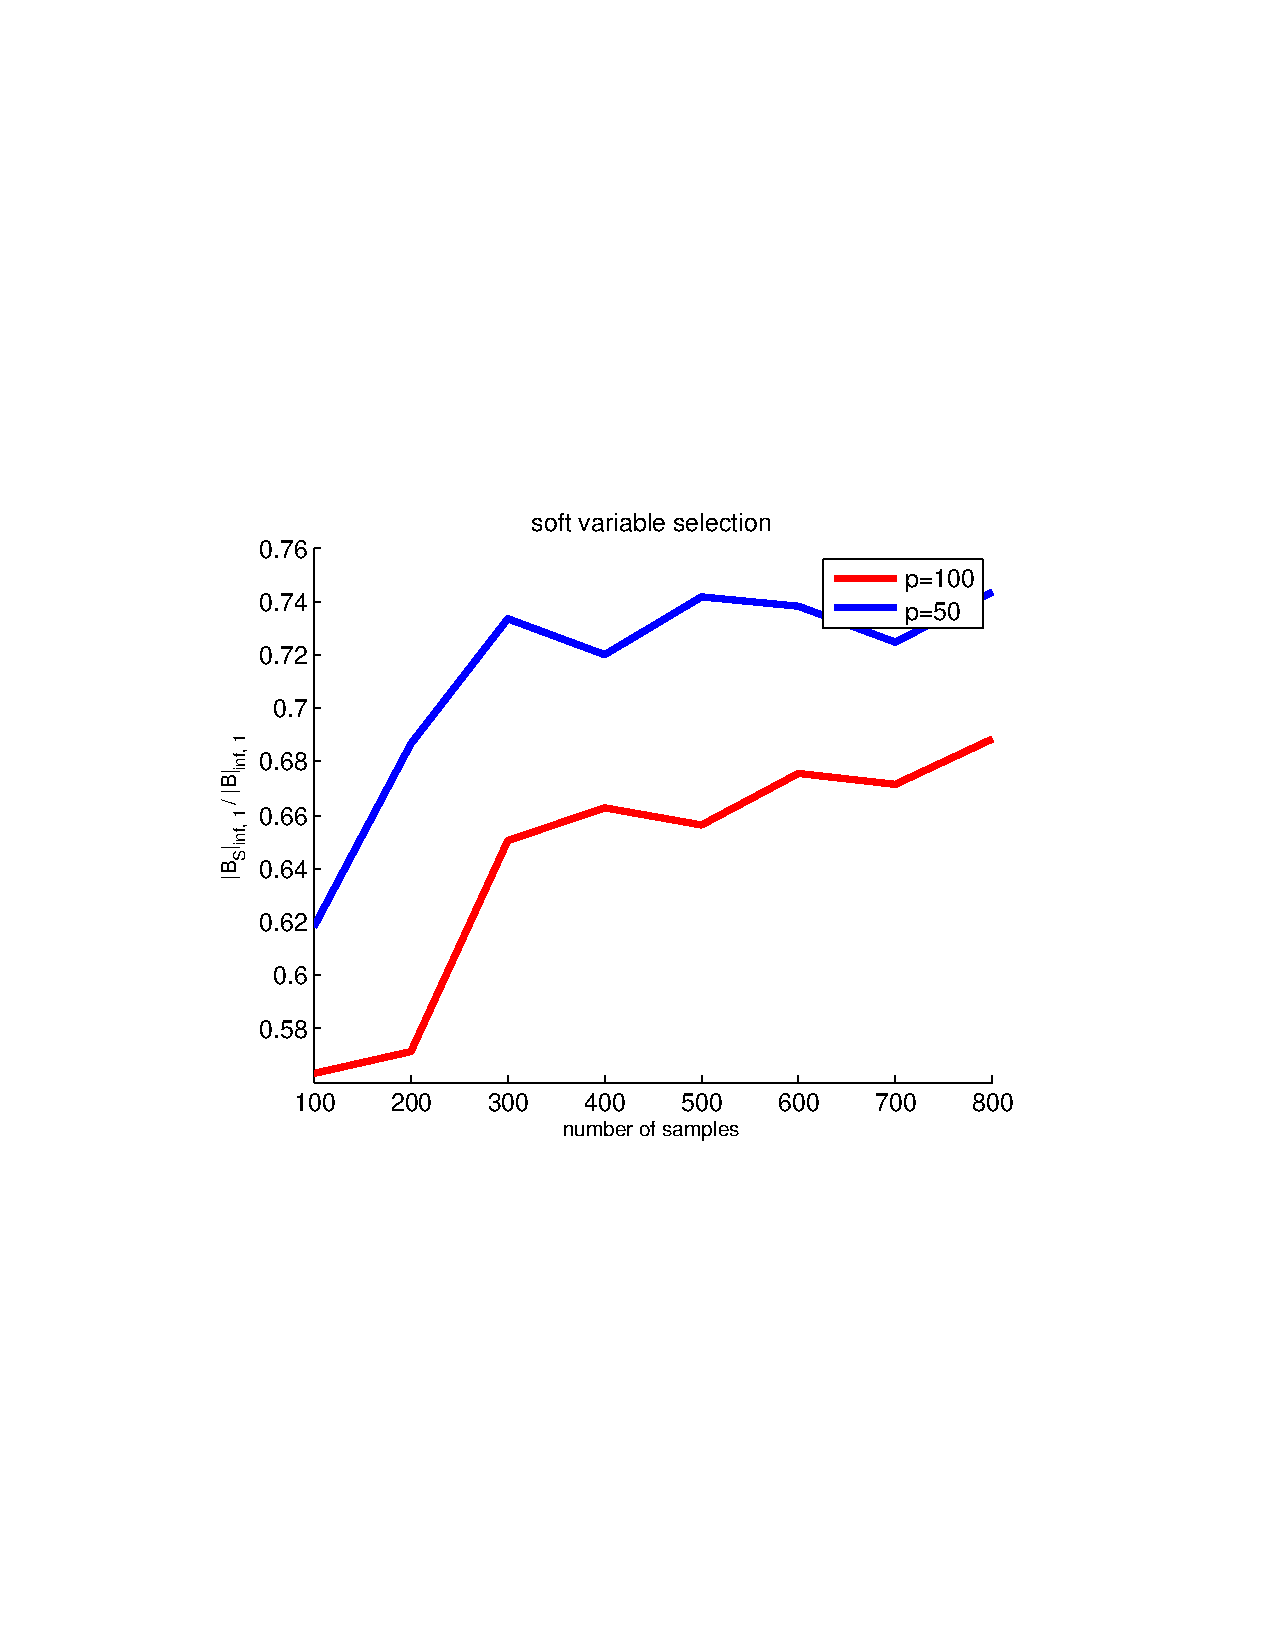
\includegraphics[trim=150 200 150 200]{../code/figs/soft_recovery.pdf}
\end{figure}
The recovery curve plateaus. It should converge to 1 but appears to be doing so very slowly.

As a thought experiment, let's consider a noiseless support recovery optimization:
\begin{align*}
& \min_B \| B \|_{\infty, 1}\\
&\trm{s.t. } y_i \geq y_j + B_j^\tran (X^i - X_j) \forall i,j
\end{align*}
The optimum of this program should become exactly sparse as $n \rightarrow \infty$, but may become sparse at a very slow rate with respect to $n$. The penalized least-square solution then, like a heat-seeking missile thrown off target by a decoy, homes in to the non-sparse optimum rather than the actual sparse solution.

We have not implemented this optimization but can still approximate it with the penalized square error optimization by setting lambda very small.

What we see if that we must weigh the dimensions to exactly recover the support. We must use a weighed form of the objective.

\begin{align*}
& \min_B \sum_{s=1}^p \lambda_s\| B_{s\cdot} \|_{\infty}\\
&\trm{s.t. } y_i \geq y_j + B_j^\tran (X^i - X_j) \forall i,j
\end{align*}

Where $\lambda_s$ is small for $s \in S$ and large for $s \notin S$. 

\begin{figure}
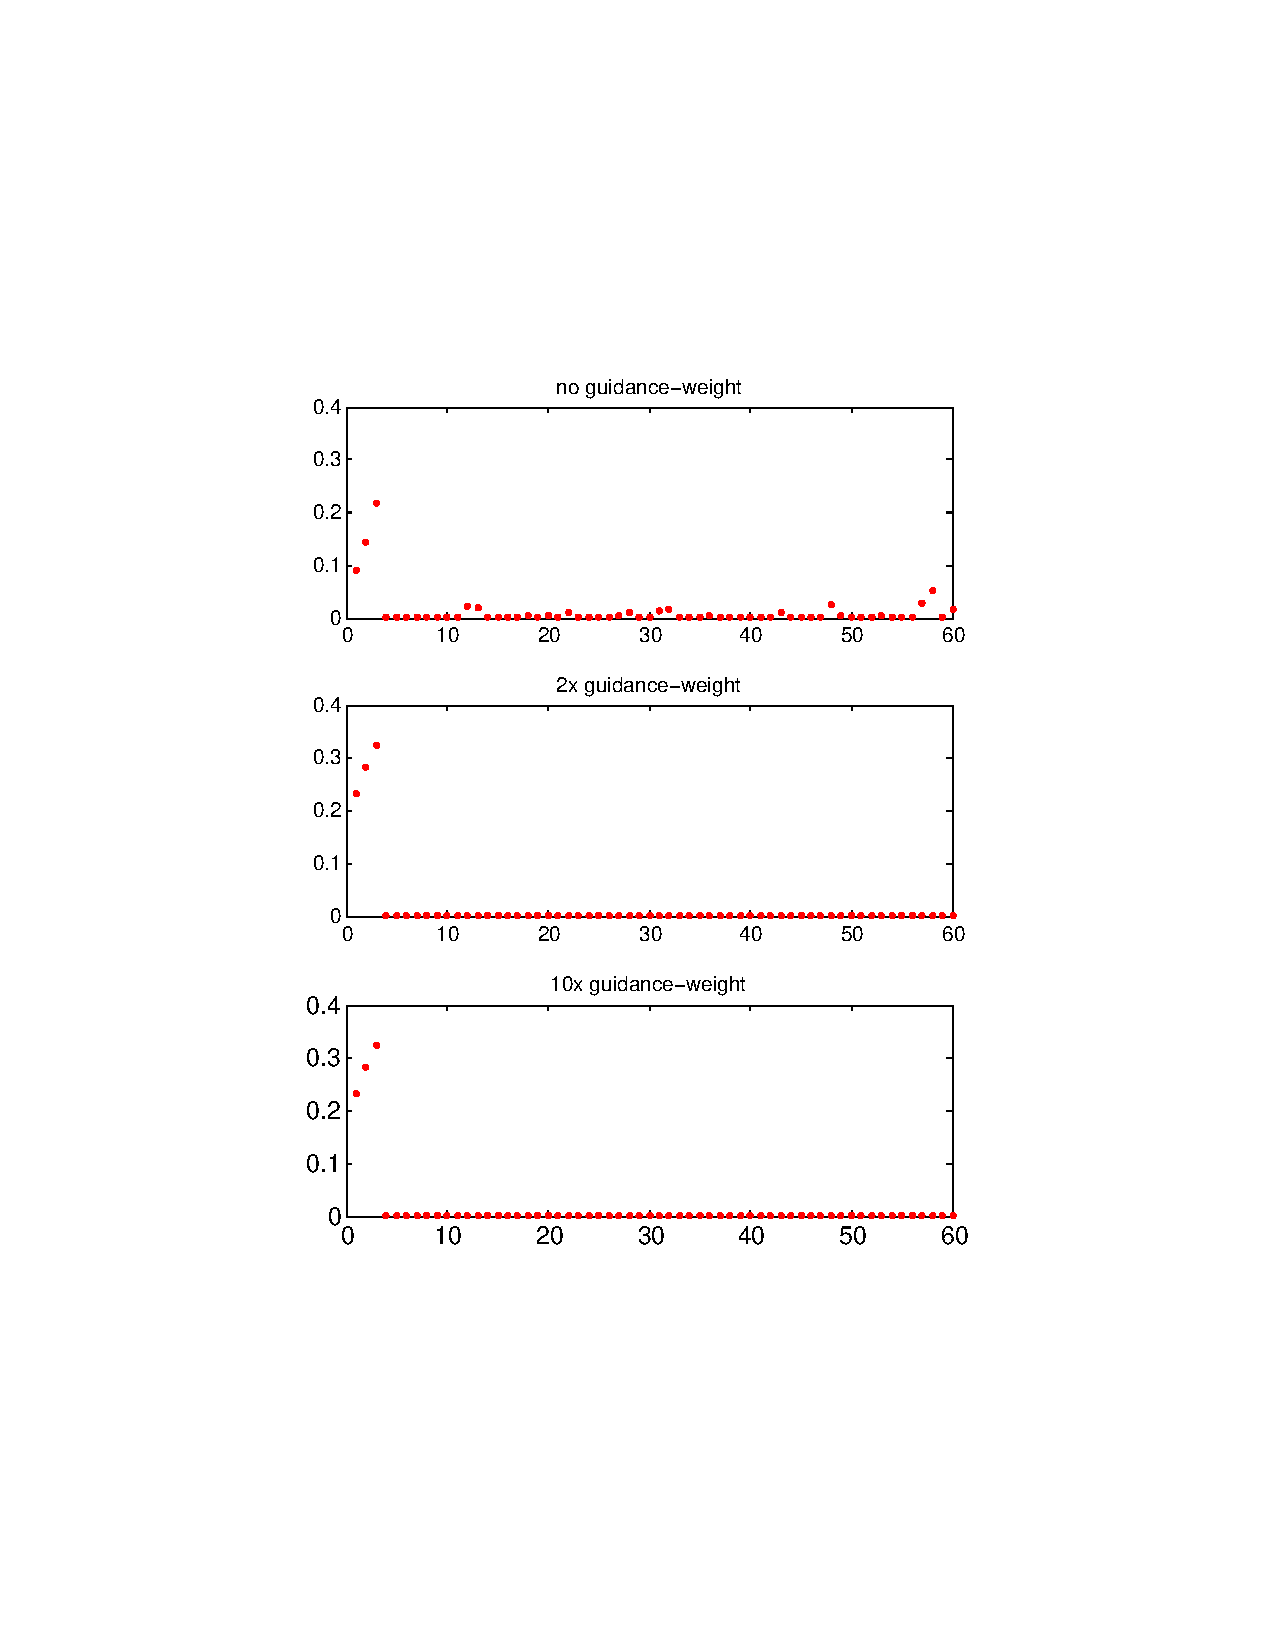
\includegraphics[trim= 150 200 150 200]{../code/figs/guided_recovery.pdf}
\end{figure}

\end{document}